\documentclass[tikz,border=6pt]{standalone}
\usepackage{ctex}
\usepackage{graphicx}
\usepackage{subcaption}
\usepackage{tikz}
\begin{document}
\begin{minipage}{0.98\textwidth}
\centering
\begin{subfigure}[t]{0.48\textwidth}
  \centering
  
\includegraphics[width=\textwidth]{real-training-images/training_curves.png}
  \caption{CAN-CNN(64x9) 训练/验证曲线}
\end{subfigure}
\hfill
\begin{subfigure}[t]{0.48\textwidth}
  \centering
  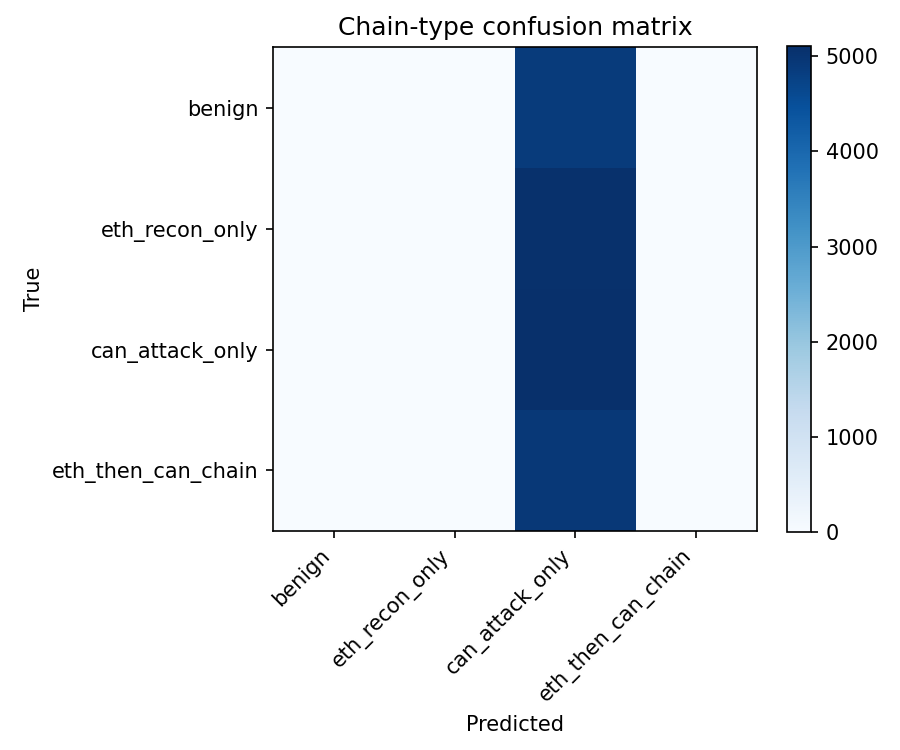
\includegraphics[width=\textwidth]{real-training-images/chain_confusion_matrix.png}
  \caption{跨域链模型混淆矩阵}
\end{subfigure}

\vspace{0.8em}

\begin{subfigure}[t]{0.48\textwidth}
  \centering
  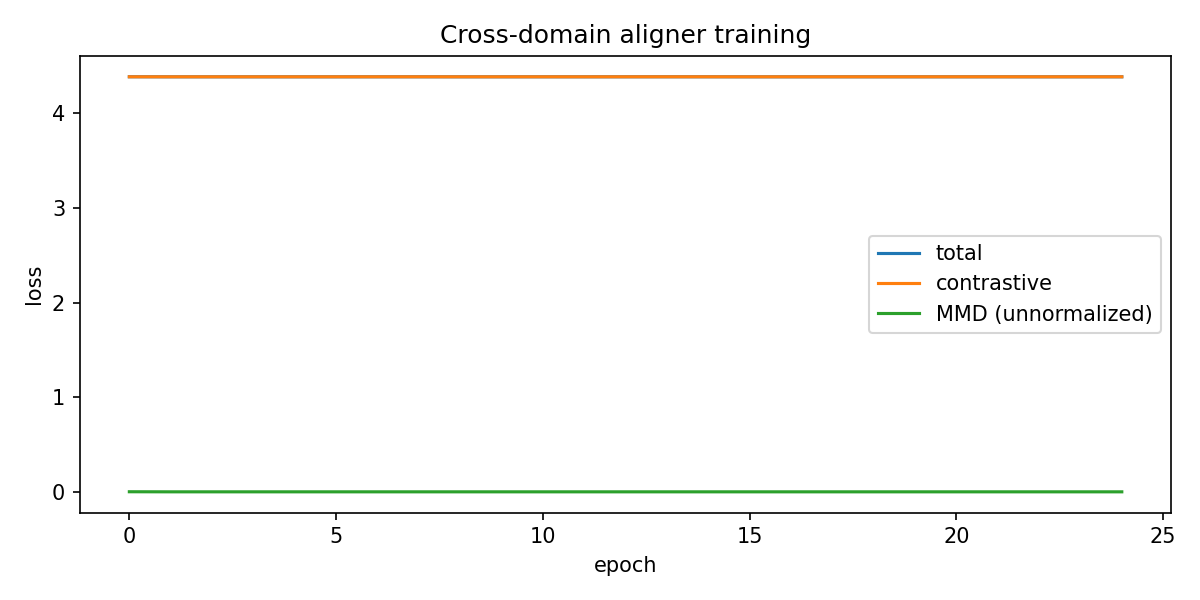
\includegraphics[width=\textwidth]{real-training-images/aligner_loss.png}
  \caption{对齐器训练损失收敛}
\end{subfigure}
\hfill
\begin{subfigure}[t]{0.48\textwidth}
  \centering
  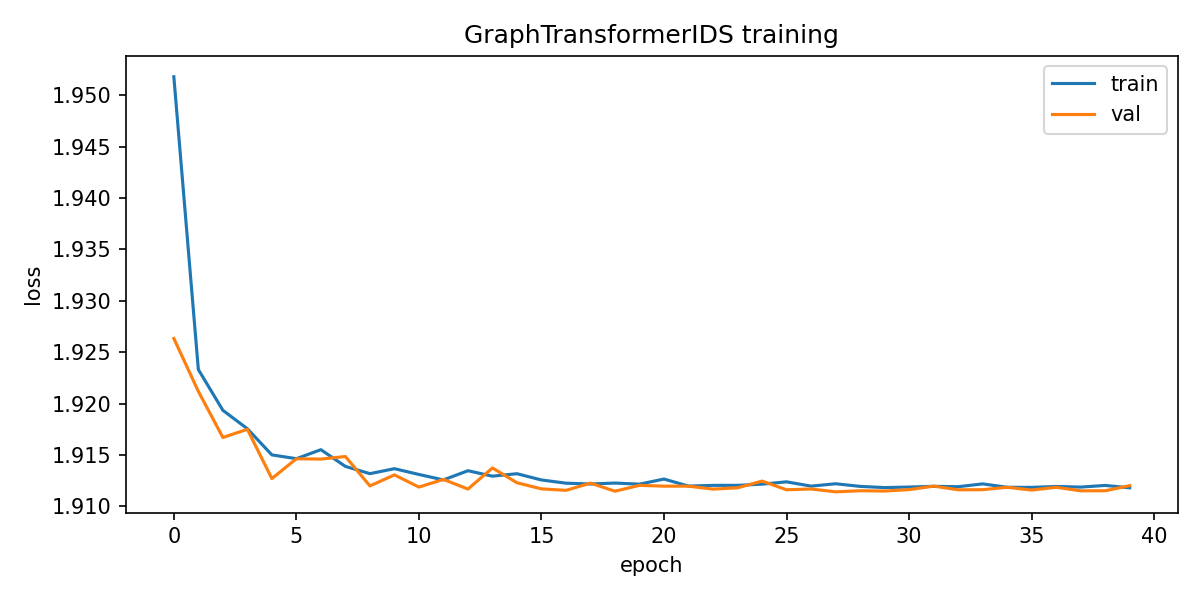
\includegraphics[width=\textwidth]{real-training-images/chain_training.png}
  \caption{链模型训练过程}
\end{subfigure}

\vspace{0.6em}

\begin{tikzpicture}
  \node[draw=black!35, rounded corners=2mm, fill=blue!6, align=left, inner sep=5pt] {
  说明：该图组全部来自实际训练产物，分别支撑“收敛性、可分性、稳定性、端到端可训练性”四个证据维度。};
\end{tikzpicture}
\end{minipage}
\end{document}
